% !TeX spellcheck = en_US
% !TeX root = ./0_article.tex

\section{Body biasing injection platforms modeling}
\IEEEPARstart{T}{he} objective of this first section is to present the work done concerning electrical modeling of integrated circuits in a BBI context.
Developing IC models in that specific case is not an easy task.
Indeed, modern digital ICs contains billions of transistors, and even considering microcontrollers where the transistor count is less important, with current technologies, it is impossible to evaluate circuits at a transistor level.

	\subsection{The hybrid simulation flow: introduction}
	To tackle these limitations, we decided to adopt an hybrid approach, combining transistor-less models and local logic gates simulations.
	This approach is a compromise between accuracy and computational cost/time, and allows simulating relatively big circuits under BBI disturbances.
	
	The resulting simulation flow is divided in three consecutive steps:
	\begin{itemize}
		\item The simulation of an IC under BBI using a transistor-less model, allowing for a purely electrical analysis;
		\item The extraction of significant disturbed signals from the previous simulation;
		\item The simulation of functional logic gates under BBI thanks to the previously extracted signals.
	\end{itemize}
	The first step allows analyzing IC macro-electrical behavior when subject to BBI, and at a lower computational cost compared to a functional model including transistors and internal transmission lines, even if it could be done in a reasonable time constraint for millions of transistors.
	Then, by extracting useful signals such as the power delivery and the transistor substrate voltages, we can evaluate what would be the behavior of actual logic gates subject to BBI.
	
	\subsection{The hybrid simulation flow : building the models}
	Building these models requires a correct understanding on integrated circuits internal structures, such as:
	\begin{itemize}
		\item The power supply network, composed of various stacked metal wires;
		\item The standard-cells, made of logic gates, and thus transistors, being pre-characterized cells used as building blocks;
		\item The silicon substrate, which can be of various type depending on the technology.
	\end{itemize}
	
		\subsubsection{Power supply rails and standard-cell segments}
		% !TeX spellcheck = en_US
% !TeX root = ./0_article.tex
% LABEL AFTER CAPTION WESH GEOFFREY !!
\begin{figure}[h]
	\centering
	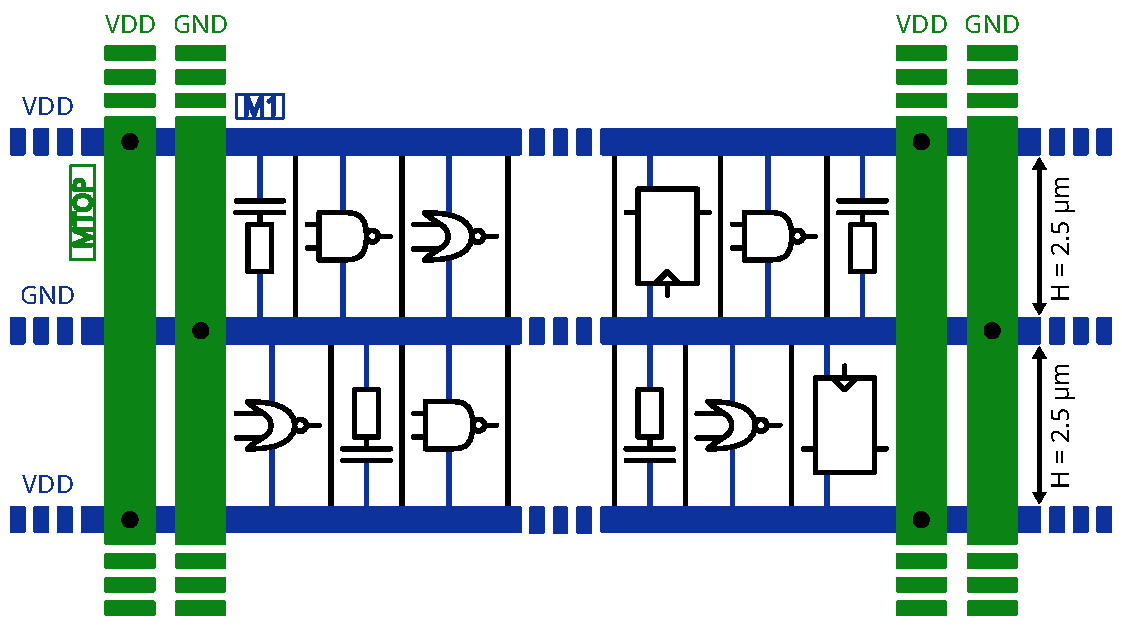
\includegraphics[width=0.49\textwidth]{./figures/psu_std_cell.pdf}
	\caption{A Standard-Cell Segment and its power delivery network.}
	\label{fig_alim_std}
\end{figure}

		The power distribution inside an IC is typically made with a grid-like structure, composed of metal wires stacked on top of each other on planes.
		The uppermost layer forms a ring surrounding the core.
		In each layer, the metal wires are equally spaced and have a dedicated width, which becomes thinner the deeper they are.
		The lowest layer brings the power directly to the transistors.
		
		Within these metal lines are located standard-cell segments (SCS), created by the power planning, as illustrated in Fig. \ref{fig_alim_std}.
		SCS are pre-characterized by foundries and classified according to their performance in timing and power consumption.
		Their height is fixed, while their width vary depending on their complexity, and are commonly made of logic gates, sequential, and decoupling elements.
	
		\subsubsection{Silicon substrate structure}
		Another important element of an IC is the substrate, and most importantly its type.
		We can mainly distinguish bulk and FD-SOI substrates.
		
		On the one hand, in bulk substrates, the transistor channel forms directly inside the P-substrate, and the depletion layer thickness is difficult to control.
		On the other hand, in FD-SOI substrates, a silicon oxide layer is created between the channel and the P-substrate, thus constraining the channel thickness.
		
		In this paper, we are focusing only on bulk substrates, and in this family, we can distinguish two substrate types: dual-well (DW) and triple-well (TW).
		The main difference between DW and TW substrates lies in how are lithographed NMOS transistors.
		In DW substrates, NMOS are located directly inside the P-doped substrate, and PMOS inside a N-doped well, called the N-well.
		However, in the case of a TW substrate, the PMOS are still inside the N-well, but the NMOS are located inside an additional P-doped well, made inside the N-well.
		
		These manufacturing differences are illustrated in Fig. \ref{fig_sub}, representing the cross-sectional view of an inverter made with a bulk technology.
		The PN and NP diodes formed between the substrate and the wells are represented, and the electrical resistances $R_C$ represent the access resistance of the substrate and the wells.
		% !TeX spellcheck = en_US
% !TeX root = ./0_article.tex

\begin{figure}[h]
	\centering
	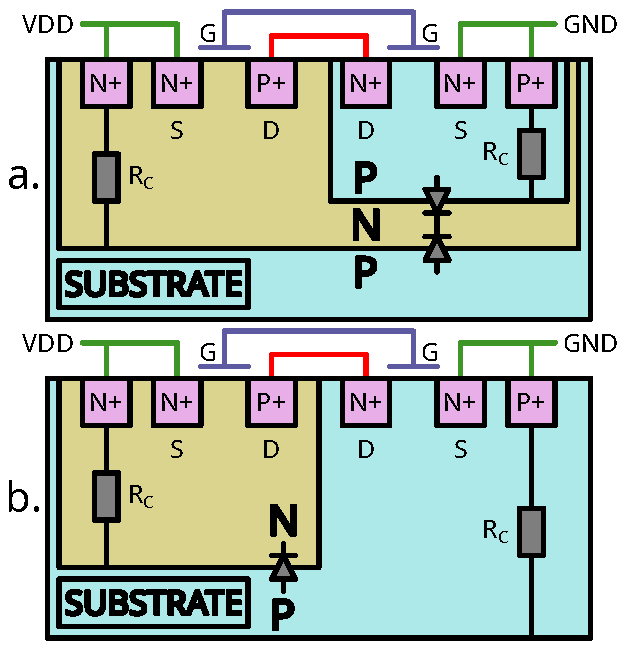
\includegraphics[width=0.35\textwidth]{./figures/substrate_2.pdf}
	\caption{Triple-well (a) and Dual-well (b) inverter cross-sectional view.}
	\label{fig_sub}
\end{figure}

		Dual-well substrates are found in moderately old ICs, while triple-well ones are common in more recent ICs, often coupled with dual-well substrate on the same die.
		The combination of both allows for \textcolor{orange}{cross-coupling noise reduction}, in addition to electrical insulation between transistors located on different domains (DW and TW).

		\subsubsection{Designing an elementary building-block for mass simulation}
		Thanks to the previously analyzed elements and models, we can now design elementary standard-cell blocks composed of the power delivery, the logic gates and the substrate, for each substrate type.
		As it has been said before, we are developing an hybrid simulation flow, therefore the designed elementary block is transistor-less.
		Eventually, our work is based on previous works on the subject \textcolor{cyan}{mathieuEMFI, FDTC2022, FDTC2023}.
		
		% !TeX spellcheck = en_US
% !TeX root = ./0_article.tex

\begin{figure*}[ht]
	\centering
	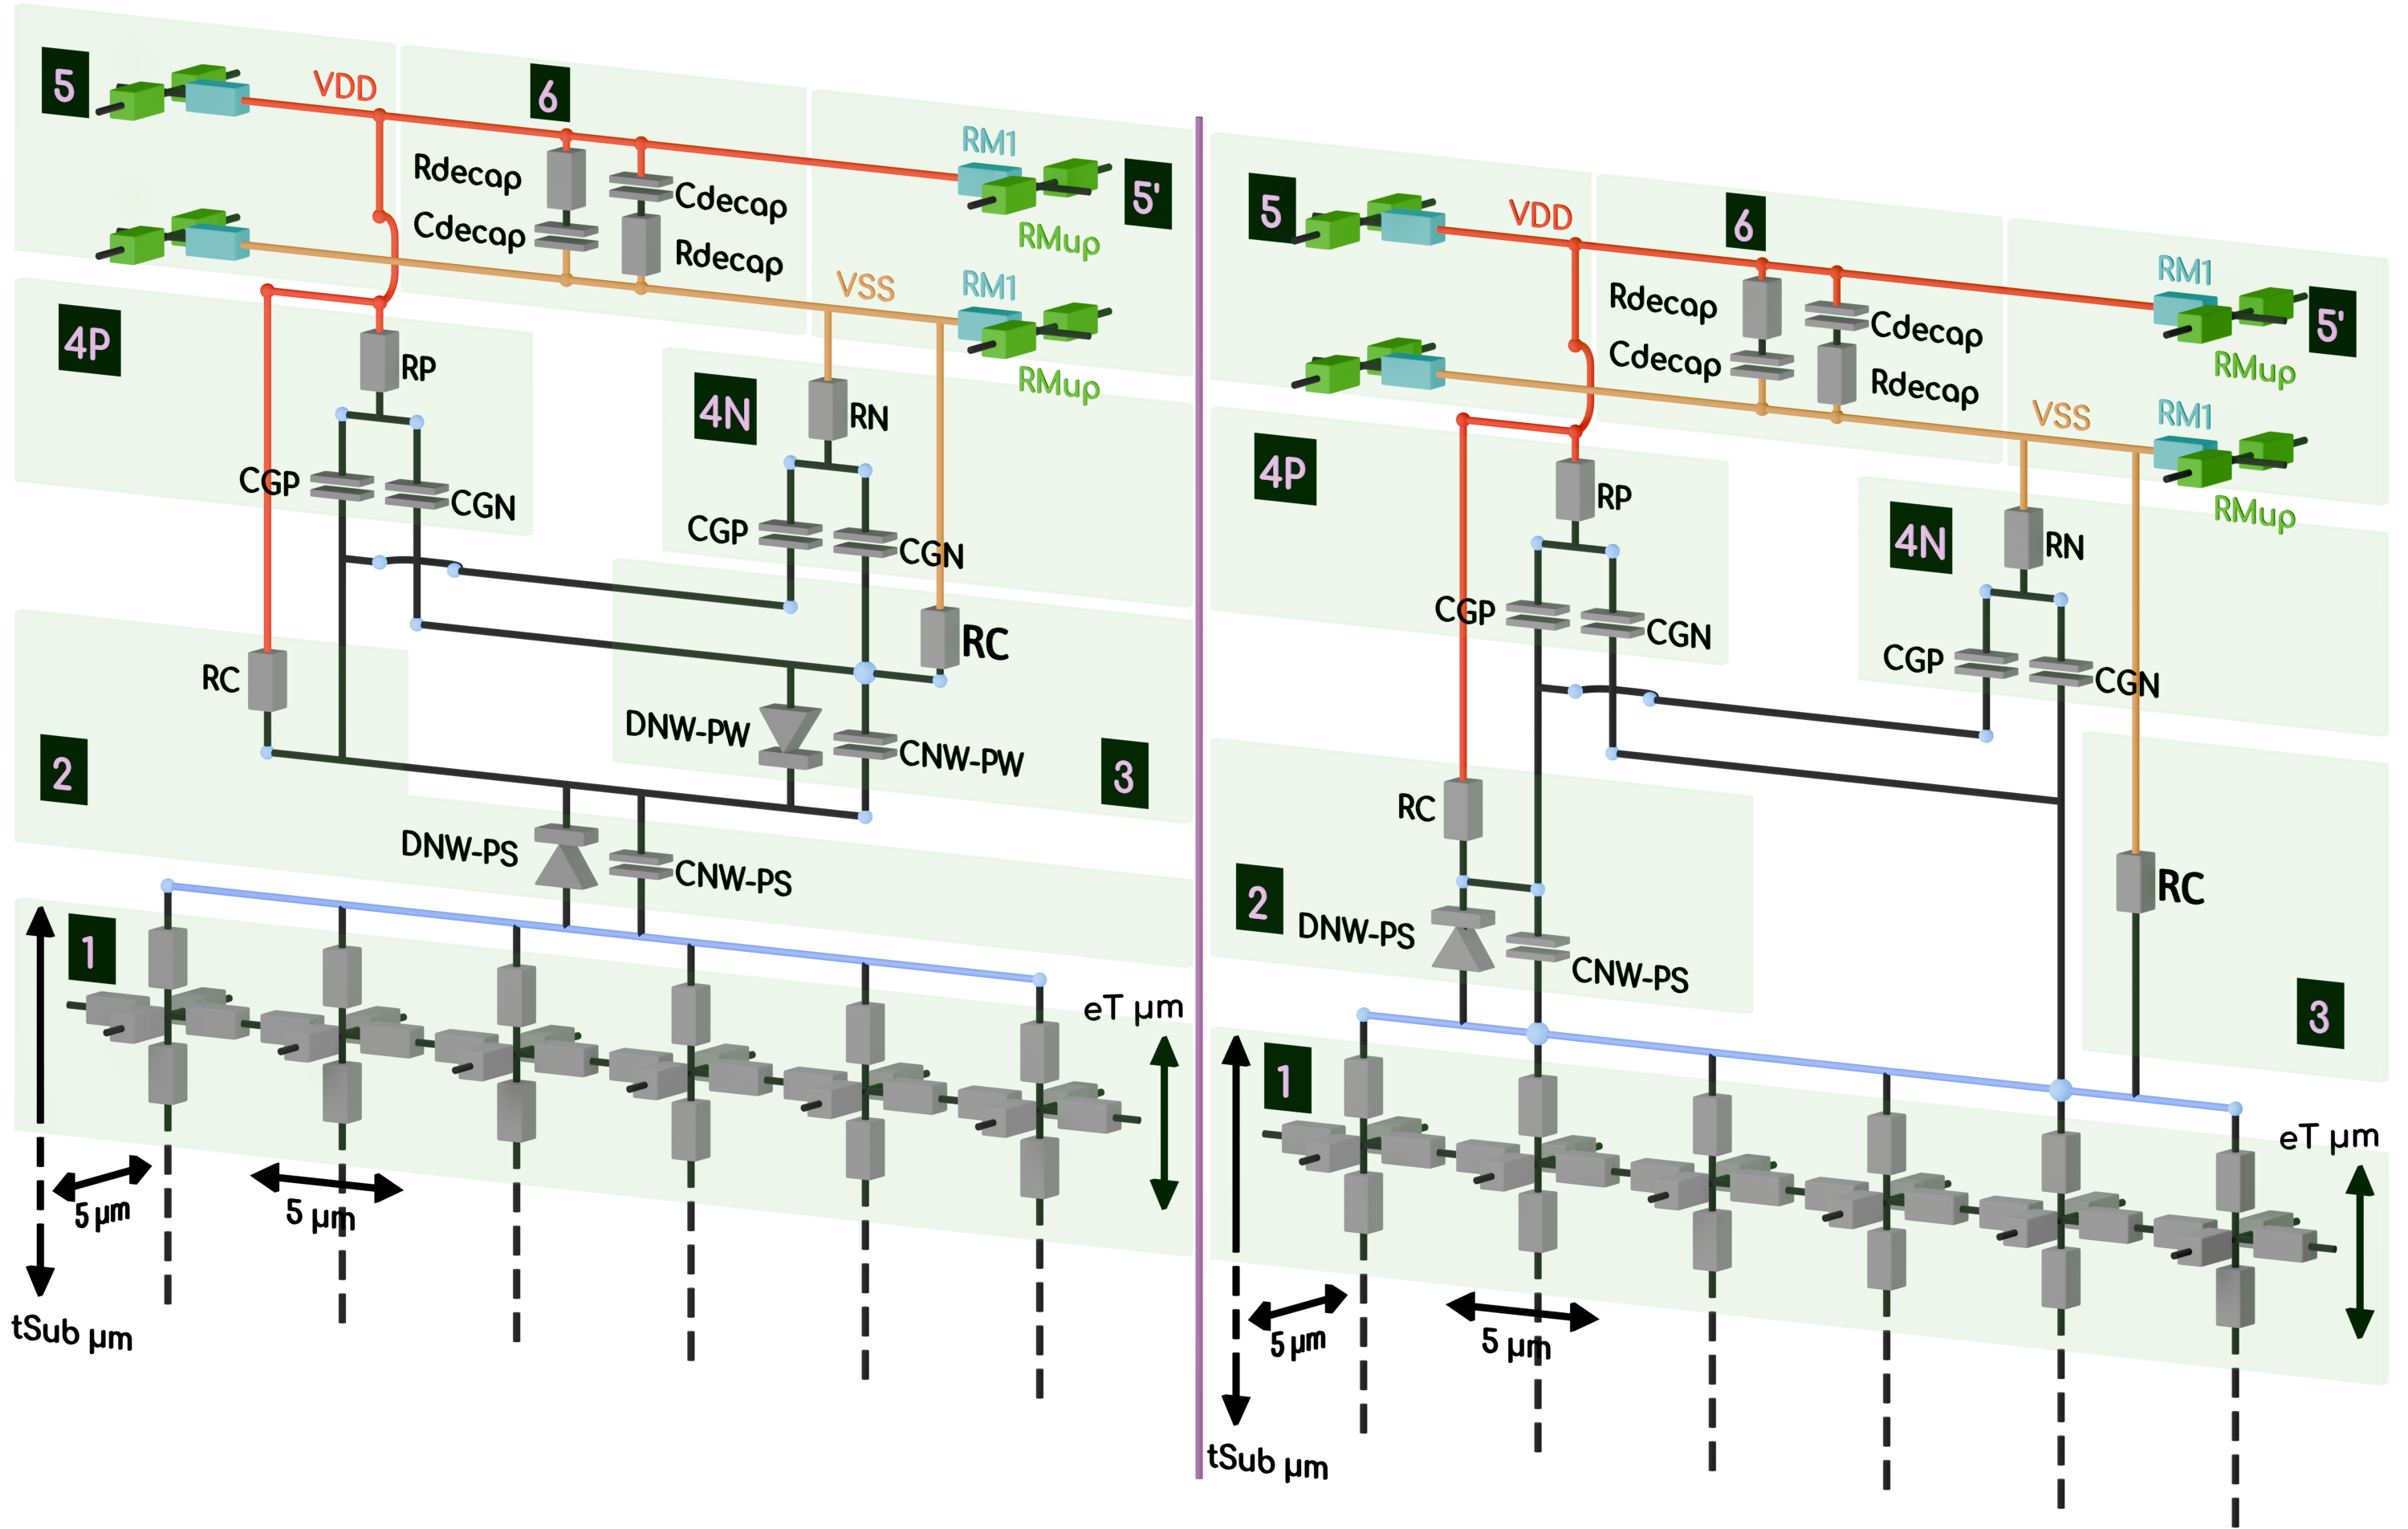
\includegraphics[width=0.95\textwidth]{./figures/dual+triple3.png}
	\caption{Triple well (left) and dual well (right) std cell \textcolor{red}{(PEUT ETRE FAIRE DES SOUS-FIGURES)}}
	\label{fig_triplewellstdcell}
\end{figure*}

		
		The model we propose is shown in Fig. \ref{fig_triplewellstdcell}.
		It represents an entire standard-cell segment, including a two levels power delivery network, average models of a hundred of logic gates, and the silicon substrate.
		For better clarity, we divided the model into 6 sections, each representing a specific building block:
		\begin{itemize}
			\item \shadowbox{1} The substrate: modeled with 6 blocks of 6 resistors;
			\item \shadowbox{2} The P-N substrate-well silicon junction;
			\item \shadowbox{3} The N-P well-well silicon junction;
			\item \shadowbox{4N} \shadowbox{4P} The MOS average electrical model;
			\item \shadowbox{5} \shadowbox{5'} The power distribution metals;
			\item \shadowbox{6} The power supply decoupling.
		\end{itemize}

%\subsection{The hybrid simulation flow : building the models}
%The transistor-less model, also called standard-cell model, is developed thanks to the internal structure of integrated circuits, including:
%\begin{itemize}
%	\item Their power supply network;
%	\item Their standard-cells properties;
%	\item Their silicon substrate.
%\end{itemize}
%These three elements and their internal structure allow elaborating average models, able to represent their macro behavior.
%Fig. \ref{fig_alim_std} illustrates the base symbolic diagram used for our design.
%It represents a standard-cell segment, composed of logic gates and decoupling elements, with a fixed height of 5 µm and a variable width.
%For simplicity, two levels of metals for the power distribution are represented, the highest level MTOP in green and the first level M1 in blue.
%
%Then, because the previous analysis does not consider the substrate on which the transistors lie, it is required to extend the model.
%To that end, we represent in Fig. \ref{fig_sub} the cross-sectional view of a CMOS inverter in a triple-well and dual-well substrate.
%The parasitic silicon diodes formed between the substrate and the N-well, and between the N-well and the P-well are represented, in addition to the wells access electrical resistances $R_C$.
%
%Thanks to these preliminary analysis and former work on the subject \textcolor{cyan}{mathieuEMFI, fdtc20222023}, we set up an elementary transistor-less model, considering every presented aspect.
%This model, shown in Fig. \ref{fig_triplewellstdcell} for a triple-well substrate, represents a column portion of an IC, being 30 µm wide, 5 µm deep, and tSub µm thick.
%The schematic is divided into 6 sections:
%\begin{itemize}
%	\item \shadowbox{1} The substrate model, an array of distributed resistors;
%	\item \shadowbox{2} The P-N substrate-well silicon junction;
%	\item \shadowbox{3} The N-P well-well silicon junction;
%	\item \shadowbox{4N} \shadowbox{4P} The MOS average electrical model;
%	\item \shadowbox{5} \shadowbox{5'} The power distribution metals;
%	\item \shadowbox{6} The power supply decoupling.
%\end{itemize}
%The passive components modeling the transistors represent about 100 hundreds logic gates in the target technology.
%Therefore, the model allows evaluating simultaneously the average electrical behavior of 100 hundreds logic gates at a very low cost.
%
%% !TeX spellcheck = en_US
% !TeX root = ./0_article.tex
% LABEL AFTER CAPTION WESH GEOFFREY !!
\begin{figure}[h]
	\centering
	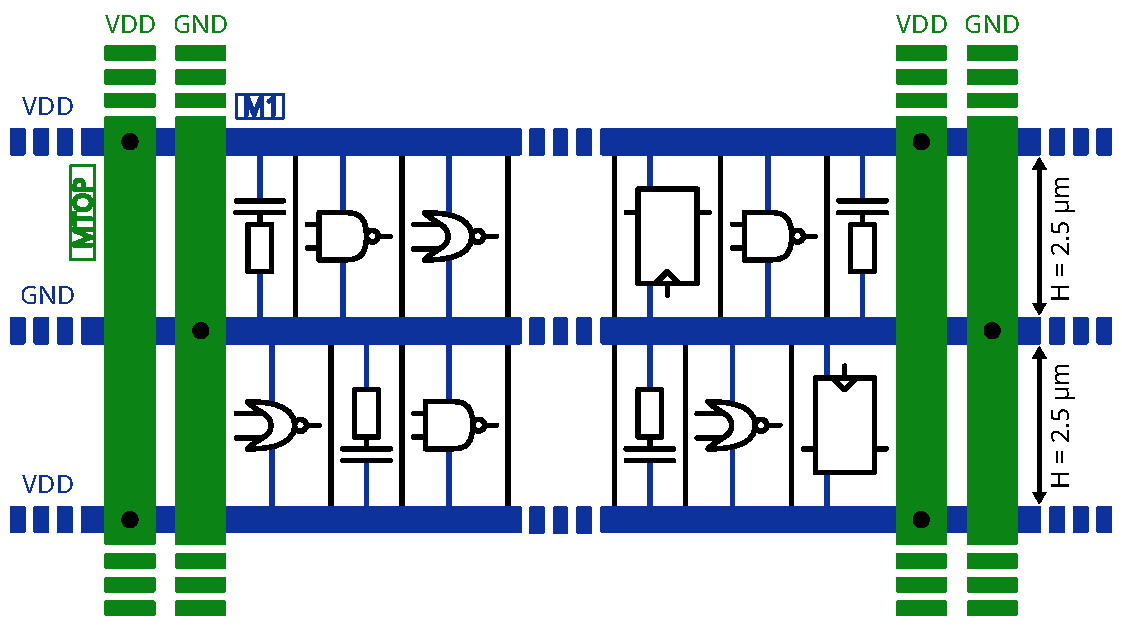
\includegraphics[width=0.49\textwidth]{./figures/psu_std_cell.pdf}
	\caption{A Standard-Cell Segment and its power delivery network.}
	\label{fig_alim_std}
\end{figure}

%
%% !TeX spellcheck = en_US
% !TeX root = ./0_article.tex

\begin{figure}[h]
	\centering
	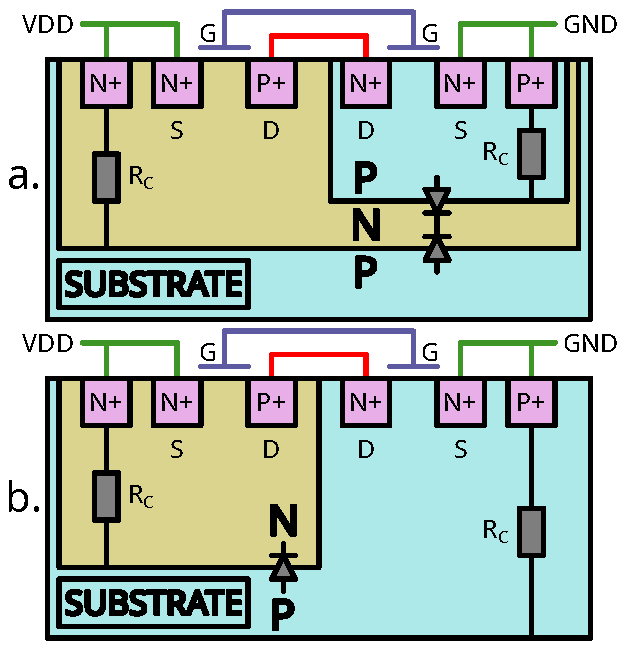
\includegraphics[width=0.35\textwidth]{./figures/substrate_2.pdf}
	\caption{Triple-well (a) and Dual-well (b) inverter cross-sectional view.}
	\label{fig_sub}
\end{figure}

%
%% !TeX spellcheck = en_US
% !TeX root = ./0_article.tex

\begin{figure*}[ht]
	\centering
	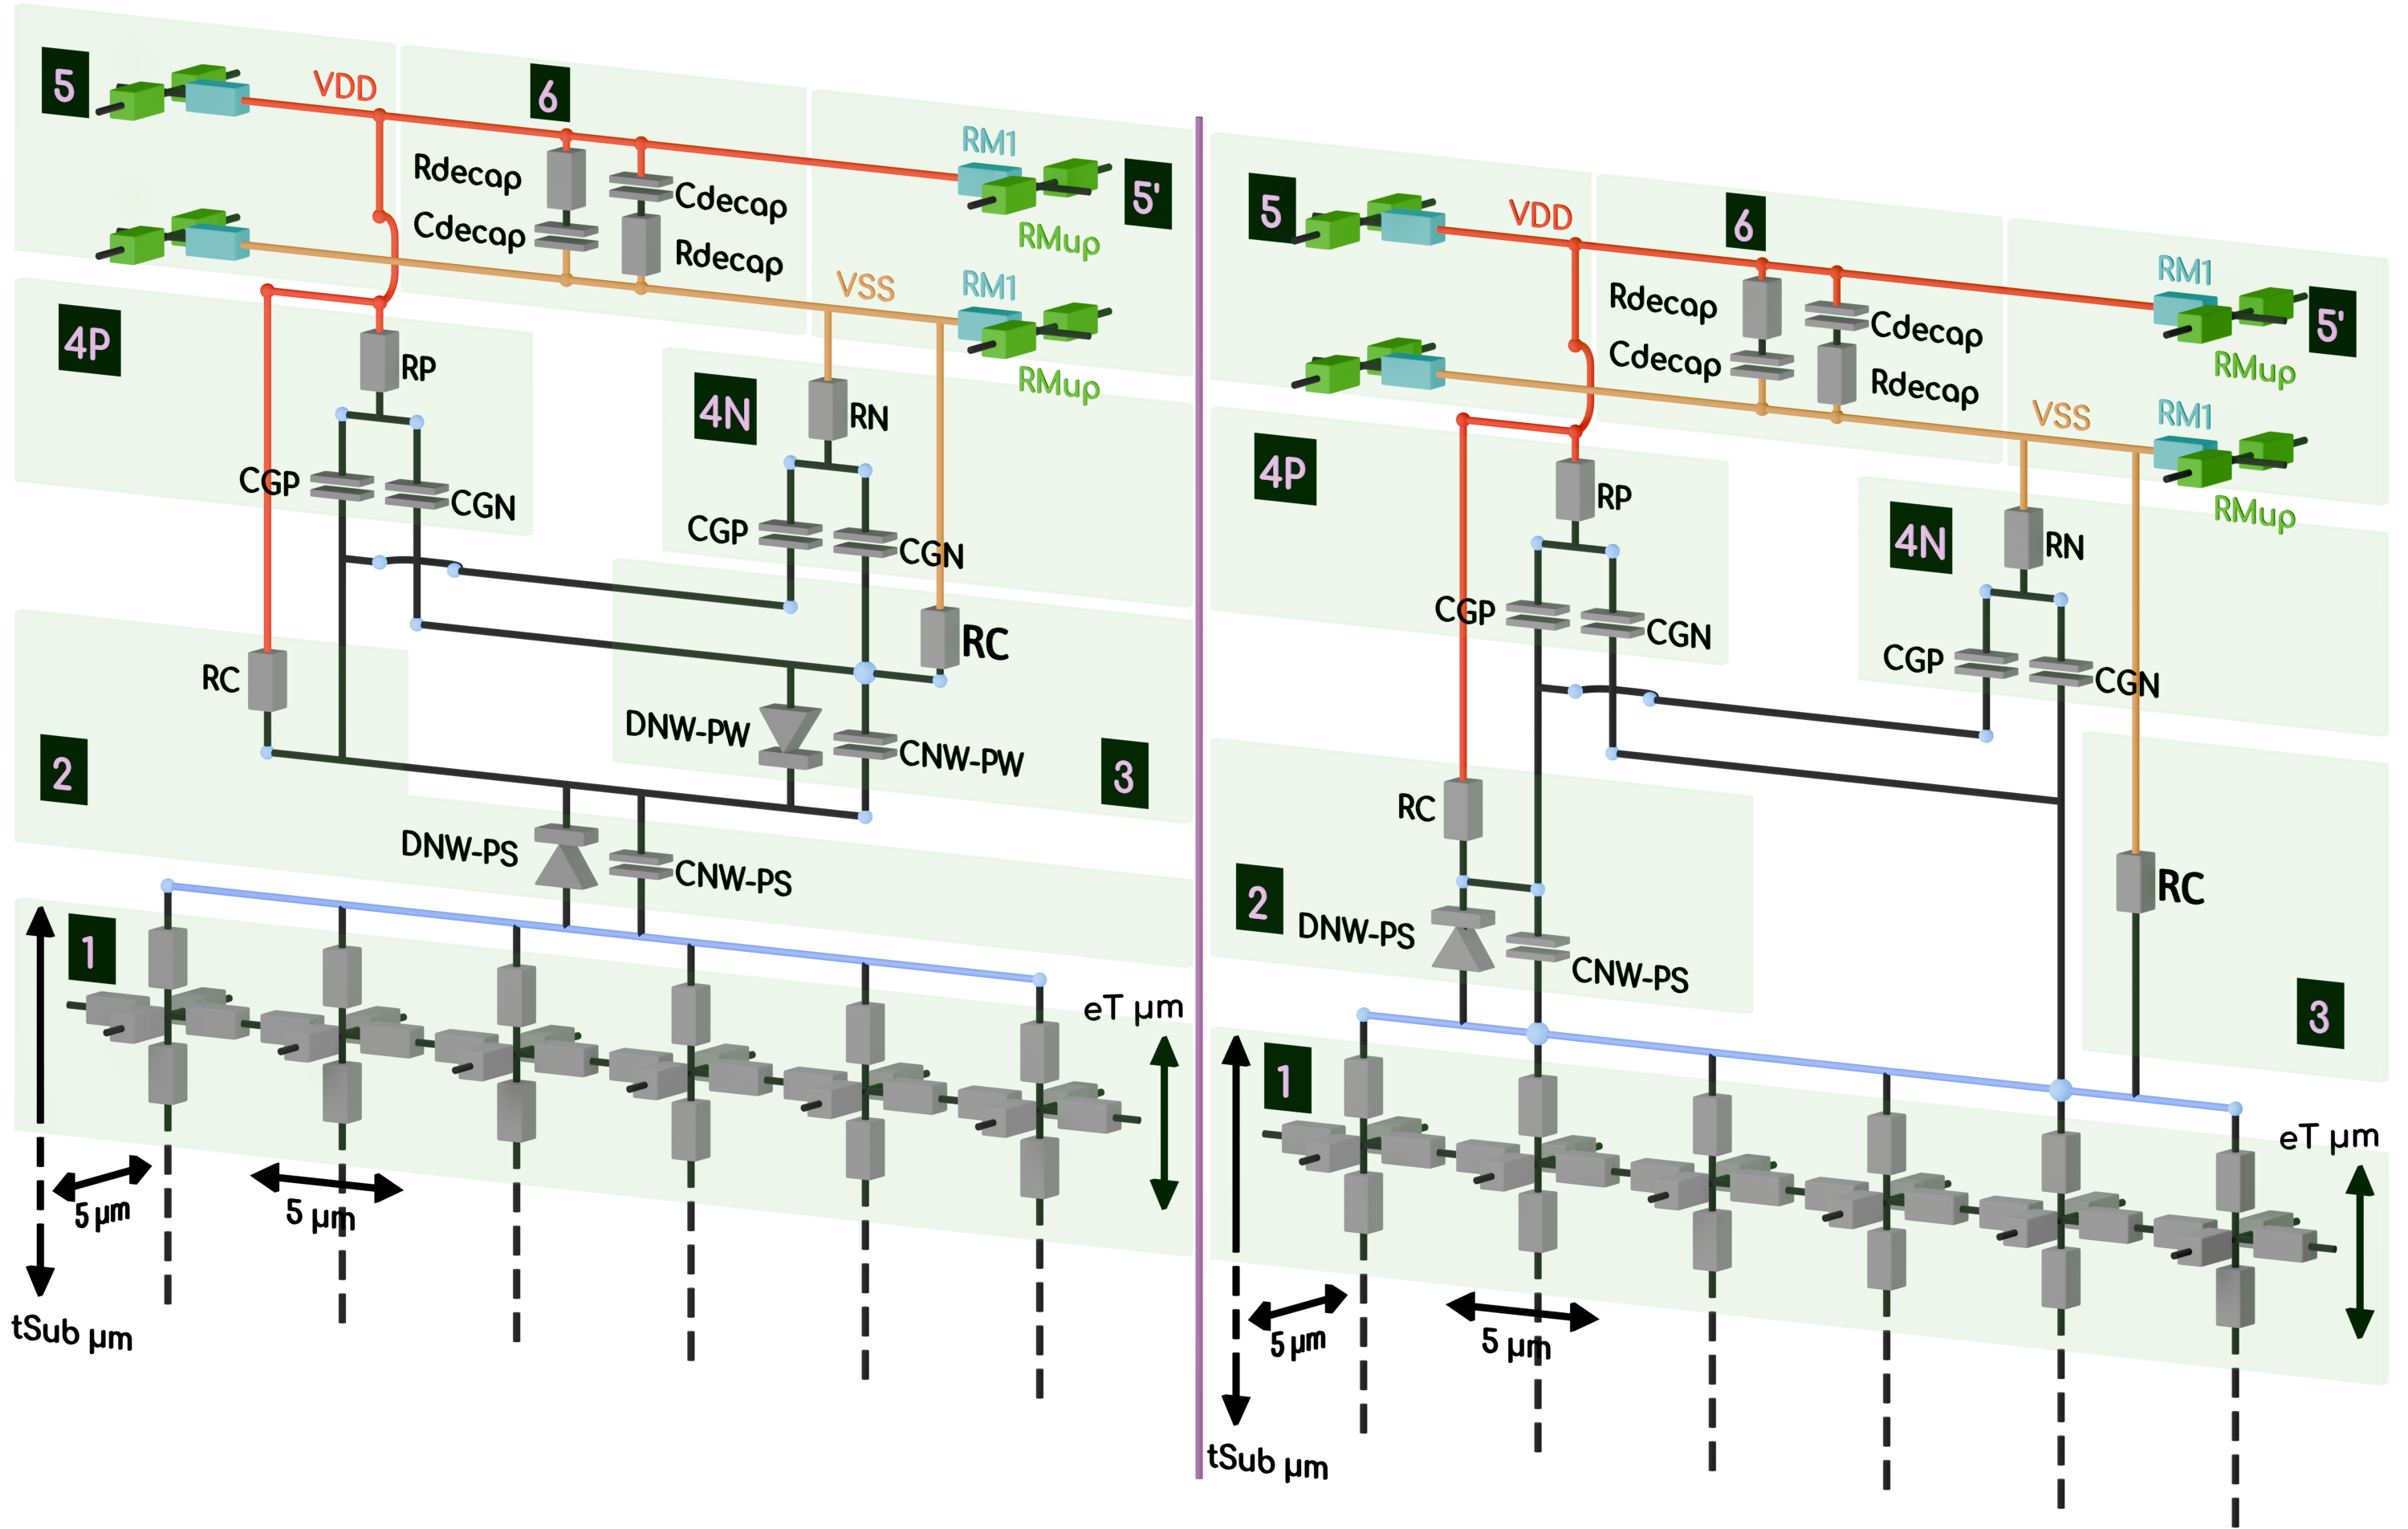
\includegraphics[width=0.95\textwidth]{./figures/dual+triple3.png}
	\caption{Triple well (left) and dual well (right) std cell \textcolor{red}{(PEUT ETRE FAIRE DES SOUS-FIGURES)}}
	\label{fig_triplewellstdcell}
\end{figure*}

